\documentclass[sigconf]{acmart}

\usepackage{booktabs} % For formal tables
\usepackage{algorithmicx}
\usepackage[ruled]{algorithm}
\usepackage{algpseudocode}


\definecolor{stringColor}{rgb}{0.8,0.1,0.1}
\usepackage{listings}
\lstdefinelanguage{JavaScript}{
  keywords={typeof, new, true, false, catch, function, return, null, catch, switch, var, if, in, while, do, else, case, break},
  morekeywords={reaction, preamble, language, actor, input, output},
  keywordstyle=\color{black}\bfseries,
  ndkeywords={class, export, boolean, throw, implements, import, this},
  ndkeywordstyle=\color{darkgray}\bfseries,
  identifierstyle=\color{black},
  sensitive=false,
  comment=[l]{//},
  morecomment=[s]{/*}{*/},
  commentstyle=\color{purple}\ttfamily,
  stringstyle=\color{stringColor}\ttfamily,
  morestring=[b]',
  morestring=[b]"
}
\lstset{
   language=JavaScript,
   backgroundcolor=\color{white},
   extendedchars=true,
   basicstyle=\footnotesize\ttfamily,
   showstringspaces=false,
   showspaces=false,
   numbers=left,
   numberstyle=\tiny,
   numbersep=5pt,
   tabsize=2,
   breaklines=true,
   showtabs=false,
   captionpos=b,
   xleftmargin=-5pt, xrightmargin=0pt
}

\newcounter{myctr}
\newenvironment{compactEnumerate}{\begin{list}{\arabic{myctr}.}
{\usecounter{myctr}
%\setlength{\topsep}{1mm}\setlength{\itemsep}{0.5mm}
\setlength{\topsep}{0.3mm}\setlength{\itemsep}{0mm}
\setlength{\parsep}{0.3mm}
\setlength{\itemindent}{0mm}\setlength{\partopsep}{0mm}
\setlength{\labelwidth}{15mm}
\setlength{\leftmargin}{4mm}}}{\end{list}}

% Copyright
%\setcopyright{none}
\setcopyright{acmcopyright}
%\setcopyright{acmlicensed}
%\setcopyright{rightsretained}
%\setcopyright{usgov}
%\setcopyright{usgovmixed}
%\setcopyright{cagov}
%\setcopyright{cagovmixed}


\copyrightyear{2019} 
\acmYear{2019} 
%\setcopyright{acmlicensed}
\acmConference[DAC '19]{The 56th ACM/ESDA/IEEE Design Automation Conference}{June 2--6, 2019}{Las Vegas, USA}
%\acmBooktitle{The 34th ACM/SIGAPP Symposium on Applied Computing (SAC '19), April 8--12, 2019, Limassol, Cyprus}
%\acmPrice{15.00}
%\acmDOI{10.1145/3297280.3297337}
%\acmISBN{978-1-4503-5933-7/19/04}



%\acmArticle{4}
%\acmPrice{15.00}

% These commands are optional
%\acmBooktitle{Transactions of the ACM Woodstock conference}
%\editor{Jennifer B. Sartor}
%\editor{Theo D'Hondt}
%\editor{Wolfgang De Meuter}

%%%%%%%%%%%%%%%%%%%%%%%%%%%%%%%%%%%%%%%%%%%%%%%%%%%%

\usepackage{amsmath}
\usepackage{amssymb}
\usepackage{subcaption}
\usepackage{multicol}
\usepackage[inline]{enumitem}
\usepackage{xcolor} 
\usepackage{ifthen}


%%%%%%%%%%%%%%%%%%%%%%%%%%%%%%%%%%%%%%%%%%%%%%%%%%%%
% Note style by Sebastian Ertel
%%%%%%%%%%%%%%%%%%%%%%%%%%%%%%%%%%%%%%%%%%%%%%%%%%%%

\newboolean{showcomments}
\setboolean{showcomments}{true} %set false for final submission
\ifthenelse{\boolean{showcomments}}
{ \newcommand{\mynote}[3]{
   \fbox{\bfseries\sffamily\scriptsize#1}
   {\small$\blacktriangleright$\textsf{\emph{\color{#3}{#2}}}$\blacktriangleleft$}}}
{ \newcommand{\mynote}[3]{}}
\definecolor{asparagus}{rgb}{0.53, 0.66, 0.42}

% One command per author:
\newcommand{\todo}[1]{\mynote{TODO}{#1}{red}}
\newcommand{\martin}[1]{\mynote{Martin}{#1}{blue}}% 
\newcommand{\marten}[1]{\mynote{Marten}{#1}{cyan}}% 
\newcommand{\isa}[1]{\mynote{Isabelle}{#1}{darkgreen}}% 
\newcommand{\ag}[1]{\mynote{Andr\'es}{#1}{asparagus}}% 
\newcommand{\armin}[1]{\mynote{Armin}{#1}{purple}}%
\newcommand{\marjan}[1]{\mynote{Marjan}{#1}{magenta}}% 
\newcommand{\edward}[1]{\mynote{Edward}{#1}{magenta}}% 


\begin{document}

\title{Actors, Time Stamps, and Determinism \\ for Time-Critical Systems}


\author{Marten Lohstroh}
\orcid{0000-0001-8833-4117}
\email{marten@eecs.berkeley.edu}
% \affiliation{%
% 	\institution{University of California, Berkeley}
% 	%\streetaddress{}
% 	%\postcode{}
% 	%\city{} 
% 	\country{USA} 
% }

\affiliation{%
	\institution{UC Berkeley, USA}
	%\streetaddress{}
	%\postcode{}
	%\city{} 
	% \country{USA} 
}

\author{Martin Schoeberl}
\orcid{1234-5678-9012}
\email{masca@dtu.dk}
\affiliation{%
	\institution{TU Denmark, Denmark}
	%\streetaddress{}
	%\postcode{2800}
	%\city{Lyngby} 
	% \country{Denmark} 
}

\author{Andr\'es Goens}
\orcid{}
\email{andres.goens@tu-dresden.de}
\affiliation{%
	\institution{TU Dresden, Germany}
	%\streetaddress{}
	%\postcode{}
	%\city{} 
	% \country{USA} 
}

\author{Armin Wasicek}
\orcid{}
\email{armin.wasicek@avast.com}
\affiliation{%
	\institution{Avast, USA}
	%\streetaddress{}
	%\postcode{}
	%\city{} 
	%\country{USA} 
}

\author{Christopher Gill}
\orcid{}
\email{cdgill@wustl.edu}

\affiliation{%
	\institution{Washington Univ., St. Louis, USA}
	%\streetaddress{}
	%\postcode{}
	%\city{} 
	%\country{USA} 
}

\author{Marjan Sirjani}
\orcid{}
\email{marjan.sirjani@mdh.se}

\affiliation{%
	\institution{M\"alardalen Univ., Sweden}
	%\streetaddress{}
	%\postcode{}
	%\city{} 
	%\country{Sweden} 
}

\author{Edward A. Lee}
\orcid{0000-0002-5663-0584}
\email{eal@eecs.berkeley.edu}

\affiliation{%
	\institution{UC Berkeley, USA}
	%\streetaddress{}
	%\postcode{}
	%\city{} 
	%\country{USA} 
}


\renewcommand{\shortauthors}{E. A. Lee et al.}

\begin{abstract}
Abstract
\end{abstract}

%
% The code below should be generated by the tool at
% http://dl.acm.org/ccs.cfm
% Please copy and paste the code instead of the example below. 
%
\begin{CCSXML}
	<ccs2012>
	<concept>
	<concept_id>10010520.10010553.10010562</concept_id>
	<concept_desc>Computer systems organization~Embedded systems</concept_desc>
	<concept_significance>500</concept_significance>
	</concept>
	</ccs2012>  
\end{CCSXML}

\ccsdesc[500]{Computer systems organization~Embedded systems}


\keywords{actor, real-time systems, worst-case execution time}

\maketitle 

\section{Introduction}\label{sec:intro}
Precision timing plays an important role in a plethora of modern systems, ranging anywhere from embedded control systems that continually interact with concurrent physical processes (i.e., cyber-physical systems) to large-scale distributed systems requiring some measure of consistency.
In order to effectively program these systems, there is a need for programming models with a semantics that includes time.
In current-day general-purpose hardware and programming languages, timing properties of software are emergent rather than specified.
Therefore, the verification of timing properties of time-critical systems relies on testing, but effectively testing software in the face of non-determinism is challenging.

In this paper, we propose an actor-oriented programming model that reduces nondeterminism by introducing a semantic notion of time, allowing programmers to specify timing properties, which, if executed on capable hardware, can be guaranteed statically.
Aimed at time-critical systems, our model is based on a discrete event semantics, which ensures that messages between actors are handled in deterministic order unless nondeterminism is introduced explicitly as a desired property.
We introduce \emph{Lingua Franca} (LF), an interface definition language for the description of actors and their composition.
LF allows programmers to implement the functionality of actors using a language of their choice.
By default, all Lingua Franca programs will be deterministic.
We achieve this using a semantic notion of time and time stamps.

% LF is designed with a pre-compilation step on polyglot principles, allowing an analysis step to make guarantees as well as opaque actors to serve as means to combine different systems. 

%This functionality will live inside actors, the interfaces of which will be described in Lingua Franca to be able to analyze global timing properties of the system. 
% Similarly desirable are guarantees, e.g. about meeting real-time deadlines, or sound properties, like determinism, which makes \emph{any} software easier to test and verify.
% However, the landscape of modern computing system is complex and very heterogeneous, which makes combining components already difficult, even more so enforcing a particular set of execution semantics. 

%is the transition here too rough?
\section{Actors}\label{sec:actor}
The actor model was introduced by Hewitt~\cite{DBLP:conf/ijcai/HewittBS73} in the early 70s. 
%A well-known programming paradigm used in this context are Hewitt~\cite{Hewitt:77:Actors} actors.
Since then,
%their introduction in the 70s,
the use of actors has proliferated in programming languages~\cite{Armstrong:96:Erlang,haller2009scala,desai2013p}, coordination languages~\cite{ren1995rtsynchronizer,ARC}, distributed systems~\cite{Hunt2018, DBLP:journals/corr/abs-1712-05889}, and simulation engines~\cite{Ptolemy:14:Book,DBLP:journals/fuin/SirjaniMSB04}.
Actors have much in common with objects---a paradigm focused on reducing code replication by means of inheritance and increasing modularity via data encapsulation---but unlike objects, actors provide a better model for \emph{concurrency} than threads, the default model for objects.
Indeed, each actor is presumed to operate concurrently alongside other actors with which it may exchange messages asynchronously. 
Objects, in contrast, are usually designed assuming a single thread of control, and retrofitting them to be ``thread safe'' is challenging and error prone.
These properties make actors ideal for programming reactive systems.
However, the lack of any guarantees with respect to the ordering of messages and the absence of a notion of time make this 
model less useful for specifying systems in which timely execution and repeatable behavior are important.

Extra machinery can be introduced for the formal specification and analysis of systems composed of Hewitt actors.
For instance, Real-time Maude~\cite{olveczky:2008:real}, a timed rewriting logic framework and (temporal) model checking tool, has been applied to actors in~\cite{Ding2003}.
Similarly, the modeling language Rebeca performs analysis that uses a model checker to ensure that nondeterminism allowed in the model does not lead to behaviors that violate requirements~\cite{DBLP:conf/birthday/SirjaniJ11}.
\marjan{, and for the timed version in \cite{KHAMESPANAH2015184}.}\marten{I would prefer to cite [102], [103], or [104] from \cite{DBLP:conf/birthday/SirjaniJ11} rather than \cite{DBLP:conf/birthday/SirjaniJ11} itself (it is a survey paper). I chose \cite{KHAMESPANAH2015184} because it is the most recent paper I could find that discusses the approach.}
Alternatively, constraints can be placed on actors' allowable behaviors so that they adhere to a well-defined model of computation (MoC), satisfying desirable properties such as deadlock freedom, schedulability, bounded memory usage, and deterministic execution, by construction. It is the latter approach that we follow.

%\ag{I tried to sum-up the big picture to help with the structure. This is based on my current understanding. It's probably not up-to-date with your project I've understood so far, so please correct me where I'm wrong.}
%
%What is \emph{Lingua Franca}? 
%\begin{enumerate}
%  \item DSL (Dual to embedded: host language gets embedded into LF)
%    \begin{itemize}
%    \item Polyglot (Multi-language)
%    \item Concrete parser
%    \end{itemize}
%  \item A MoC (refining of actors)
%    \begin{itemize}
%    \item Formal specification
%    \item Concrete implementations (hosts)
%    \end{itemize}
%  \item An analysis Framework
%    \begin{itemize}
%    \item Annotations ``implicit'' from language
%    \item Concrete reasonings (e.g. WCET analysis?)
%    \end{itemize}
%\end{enumerate} 
%
%Advantages:
%\begin{enumerate}
%\item Multi-language and multi-system: allows combining (``glue'') and reuse of legacy systems and code.
%\item Concurrency and determinism.
%\item Encapsulation via scoping mechanisms.
%\item Analysis through interface definitions.
%\item A semantic notion of time.
%\end{enumerate}

%\section{Actors in Lingua Franca}
% sectioning.... ?
\section{Lingua Franca}
In the original Hewitt actors and many modern implementations, actors have references to the actors that they communicate with.
In Lingua Franca, rather than addressing each other directly, actors exchange messages via ports. This level of indirection allows actors to be agnostic to the presence or absence of their counterparts. The connections between actors are embedded in a level of hierarchy---a composite---that is responsible for transporting messages between contained actors. While this approach increases modularity and, more importantly, exposes dependencies between actors.
These dependencies can be used to devise a schedule that ensures that (1) actors observe produced messages in time stamp order, and (2) actors cannot produce messages with a time stamp $t$ until all anti-dependent inputs with time stamp $t$ are known. This is the approach taken in the Discrete Event implementation of Ptolemy II~\cite{LeeEtAl:7:DiscreteEvents}, which is formally based on a synchronous/reactive MoC~\cite{LeeZheng:07:SRDECT}.
To increase efficiency, our approach avoids performing a fixed-point computation by executing actors in topological order. That way, each actor is only executed at most once per tick of the logical clock. Because the schedule is based purely on the topology of the actor graph, no static analysis of the actors' internals is required---Ptolemy actors are treated as black boxes.
Dynamic changes in the topology are handled hierarchically, so that the extent of the graph that is subject
to rescheduling is contained when mutations occur during runtime.
A runtime mutation always occurs within a composite actor whose interface remains unchanged.
%\marjan{and this is built based on the assumption that we have a static topology.}

% also, no need for postfire % maybe mention that this optimization comes at the loss of the ability of handling some zero-delay feedback models...
\edward{This paragraph needs work.}
LF actors, on the other hand, are better characterized as \emph{gray} boxes considering they reveal some key features of their internal structure, namely a closer approximation of the true dependencies between their ports. 
\edward{This is not quite right. The causality interfaces of Ptolemy II (Zhou et al.) expose fine-grain causality information.}
Other than actors in Ptolemy II, which implement an abstract semantics~\cite{TripakisEtAl:12:AbstractSemantics} that requires each actor to perform all of its computation in a so-called \emph{fire} function, LF actors are broken down into smaller units we call \emph{reactions}. This approach, inspired by the characterization of dataflow processes given in \cite{LeeMatsikoudis:09:Dataflow}, exposes the dependencies between actors' inputs and output at a finer grain. We enforce simple lexical scoping rules, which virtually any programmer is already familiar with, to limit reactions' access to the actors' input and output ports, thereby eliminating dependencies between ports that are out of scope. 

The interface definitions of reactions are much like function definitions. Consider the following example which defines a brake component as an LF-actor:
\edward{A brake component is probably not a good example for an ECMA 6/Flow target language. The target language should be C, or a web example should be chosen. Also, this example won't compile. What is ``pressed''? Also, ``state'' needs to be set in initialize. Also, our current syntax terminates lines with semicolons.}

\begin{minipage}{0.50\linewidth}
% \begin{enumerate}
%   \item First item \\
%         This is the second line in item and this may extend to third if long
%   \item second item\ldots
% \end{enumerate}
\begin{lstlisting}[numbers=none]
language ECMA6/Flow;
actor Brake {%
  input check:any
  input apply:number
  output on:boolean
  preamble 
\end{lstlisting}
\end{minipage}%
\begin{minipage}{0.50\linewidth}
\begin{lstlisting}[numbers=none]
  reaction(apply) -> 
  reaction(check) -> on 
%}
\end{lstlisting}
\end{minipage}%

\todo{Explain this, discuss polyglot}
\todo{Precisely because no static analysis is required...}

Having this finer-grained dependency information available at the interface level also opens up avenues for scheduling optimizations, makes the detection of zero-delay feedback less conservative, and, we conjecture, will enable remote procedure calls (RPCs) between actors without compromising determinism or modularity. 
The same dependency analysis performed to devise a schedule for message delivery and rule out zero-delay feedback can also be used to coordinate RPCs and guarantee deadlock freedom. We think that integrating RPCs into LF will be key to achieving wide adoption of our programming model, because it is such an omnipresent language feature, even in some actor-based frameworks, for example Ray~\cite{DBLP:journals/corr/abs-1712-05889}.
\marjan{When you have atomic execution of reactions, then what does RPC mean? what is the difference between an RPC and Call-Backs (or maybe callbacks with priorities)? Maybe we just leave this out for this version of the paper?}
\edward{I agree that this does not say enough to be understandable. An example would be needed.}
\martin{Do we really want to introduce RPC between actors in this paper? Isn't it syntactic sugar?
We probably do want to introduce RPC with a callback to the outside world (the HTTP get example),
like in the accessors world.}

Central to the LF programming model is the relationship between the time stamps of messages.
These time stamps denote \emph{logical} time, and the essential semantic feature is that every actor sees messages in time-stamp order.
When an actor receives multiple messages with the same time stamp, these messages are logically
\emph{simultaneous}, and the actor handles them in a well-defined deterministic order.
Logical time is distinct from physical time, as measured anywhere in a networked application.
First, logical time remains constant during the execution of any reaction in any actor, and outputs produced by that reaction have
the same logical time stamp as the inputs that trigger the reaction.
But in LF, there is a relationship between logical time and physical time,
a relationship that helps to reliably deliver real-time behavior.
\edward{This relationship needs to be explained more carefully and using examples. The following is just going to be confusing. I suggest deleting it and explaining later.}
The passing of \emph{physical} time, approximated by the system time of the execution platform. While logical time can be sped up or slowed down arbitrarily in a simulation, the fact that actors can interact with the physical world through sensors and actuators requires that logical time and physical time ``keep up'' with one another in order to have a temporal semantics that obeys the principle of causality (i.e., effects cannot precede causes) for all observers. 

% Sort reactions topologically based on precedences.

% Global notion of “current time” t.

% Event queue containing future events.

% Choose earliest time stamp t’ on the queue.

% Wait for the real-time clock to match t’.

% Execute actors in topological sort order.

% \begin{figure}[ht]
% \begin{algorithmic}[1]
%  \Procedure{execute}{}
   
%  \EndProcedure
%  \end{algorithmic}
% \caption{The Lingua Franca execution engine \marten{Maybe too much detail}}
% \label{fig:lf-engine}
% \end{figure}

% Time is \emph{logical} time. This logical time be used for simulation and then
% we call it model time. We can also use the network of actors for the implementation
% of the system. 

% In that case wall clock time is used to timestamp input values
% at sensors. Logical time can never advance further than wall clock time.
% We have a notion of delay in two places: (1) as a delay actor to break up
% feedback loops (2) at actuators to specify that an actuation shall happen before
% (or exactly at) the logical time of the input plus the delay.

% Actors communicate via ports. All data exchanged has a timestamp.
% An actor does not advance time, the reaction is considered instantaneous.

% Reactions of one actor are atomic and are allowed to change state.
% Reactions are triggered by available inputs with timestamps at logical
% time (or older). When several reactions of an actor are enabled at the
% same time, the definition order in LF defines the execution order.

% A reaction of an actor can also be released by a trigger. A trigger
% can be periodic triggers or a single shot timer.
%The engine that drives the execution of LF actors (see Figure~\ref{fig:lf-engine}) enforces the following principles:
We summarize our model in terms of the following principles:

\begin{enumerate}
\item Messages exchanged between actors are timestamped and denote a discrete event.
\item Actors have input ports, triggers, output ports, state, and an ordered list of reactions.
\item A reaction is a procedure, and any two reactions of an actor are mutually exclusive; they execute atomically with respect to one another;
\item Each reaction declares the input ports and triggers to which it reacts and to which output ports it may write.
\item If a reaction declares that it reacts to multiple input ports, then at the time of the reaction, at least one of those
input ports will have a message time-stamped with the time of the reaction, but the other input ports may be \emph{absent}
(no event is present at this logical time).
\item A reaction must also declare inputs that it does not react to but that it reads;
at a logical time, those inputs may also be absent.
\item At each logical time for which there is an input message or trigger, all reactions to those inputs and triggers will be invoked in the order in which the reactions are defined.
\item Logical time is constant during execution of a reaction.
\item For each reaction, logical time is strictly increasing; that is, a reaction will never be invoked at a logical time that is equal to or less than that of a previous invocation.
\item A reaction can schedule a trigger at a future logical time.
\item A reaction can read and modify the actor's state.
\item A reaction can set the values of the output ports that is it has declared, and if it does so, a message will be sent after the conclusion
of the reaction with a payload equal to the final value set by the reaction.
\item If multiple reactions write to the same output port, then the message sent will be that set by the last reaction invoked.
\item No two distinct actors may send messages to the same input port of another actor;
a composition of actors that does this is an erroneous composition.
\item An output port may send messages to multiple input ports or multiple actors;
these messages all bear the same time stamp.
% \edward{Note that this has dependency implications... An output message cannot be sent until the last reaction declaring that output has had a chance to run.}
\item At a logical time, a reaction may read inputs that are not triggering inputs, but it must declare that it reads those inputs,
and those inputs may be \emph{absent} (no event is present at this logical time).
\item \martin{We are not talking about delay here, but logical time is constant during reaction. There is no explicit
mentioning that the output time stamp is the same as the input time stamp (except when having a delay on
a reaction).}\marten{If we implement Delay using an actor that self-schedules a delayed reaction, the claim that no time passes during a reaction still holds.}
\end{enumerate}

\marjan{Maybe a classification of above principles makes the presentation nicer, just maybe some titles (and maybe some shuffling), like trying to go top-down, first talking about Actors, then body of reactions, then how reactions are triggered and ... and finally composition of actors ...}
\marjan{You say: We have input message or trigger; a reaction must also declare inputs that it does not react to but that it reads; now, if we have an input message at some model time but no triggers, nothing will happen until a trigger is there, right?}

Together, these rules ensure that the execution of a composition of actors is deterministic
in the sense that given any set of time-stamped inputs from outside the composition, the composition has exactly one behavior.
This determinism can be proved by showing that at each logical time, every actor realizes a monotonic function in an appropriately
chosen partial order and that the execution converges to a least fixed point in this partial order~\cite{LeeZheng:07:SRDECT}.
Within these rules, there are various opportunities for ``syntactic sugar,'' where complex behaviors can be expressed
more compactly, for example with the Ptolemy II notion of ``multiports'' or ``persistent ports'' \cite{Ptolemy:14:Book}.

%\martin{ We have discussed two different input ports:
%those that are only valid during the logical time of the time stamp (what did we call them?)
%and the ones that latch the value and are valid in future logical time as well.}
%\marten{I think we called them input ports and triggers, respectively. See item (3)(a). If unclear, we should definitely improve the wording. Same for the terminology. We could also go for external/internal input ports. Internal ports are only referenced by the actor itself; both can be considered triggers...}
%\martin{I don't think this is trigger. An input port may be part of a trigger, and for the ones that are only valid
%during the local time need to be part of a trigger condition. Otherwise they would not make any sense.
%The discussion came on what is the meaning when a reaction uses two inputs, but only one is
%triggering it. What is the value of the other: either absent or the last value (the latching input).
%That latching input needs a default value. And that is actually the way to specify it in the accessors
%framework (according to Edward, I have not checked).}
%\marjan{So, do we have two types of ports? one can only accept "events" and other can only accept "values"?}
%\martin{Both types are ``events'' with a time stamp that can trigger a reaction. The question is when
%a port is read that has not an event with the current logical time: is the content just ``absent'' or does it
%have the ``last seen'' value. I think both might be useful. Although it is probably syntactic sugar.
%The latching port can be simulated by a trigger on the input and storing the value in the state of
%the actor. Maybe this would be a leaner and cleaner semantic.}
%\marjan{Ok, I think I understand what you mean. And I am just thinking, sometimes we need to know if the event at the other port is "new" or not too old, can we do that here? I guess we can write a code for that, keeping the "model time stamp" of the "last seen" value maybe ... }

\section{Timing and Determinism}
\todo{discuss timing and scheduling using actor graph examples (no code)}
\subsection{Delays and Deadlines}
$\mathcal{D}$
We have a notion of delay in two places: (1) as a delay actor to break up
feedback loops and (2) at actuators to specify that an actuation shall happen before
(or exactly at) the logical time of the input plus the delay.

Delays deserve also the purpose to align events with wall clock time and to
allow execution of reactions in their worst-case execution time (WCET).
The sum of all reaction's WCET from one synchronization point (either
sample of sensors or output of a delay actor) to another synchronization
point (or output of an actuator) has to be less than the delay.
\begin{figure}[ht]
 \centering
 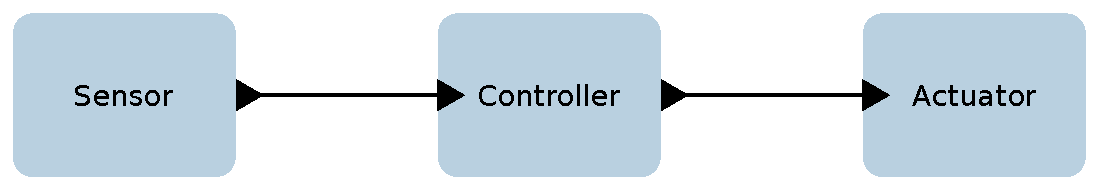
\includegraphics[width=\linewidth]{img/example-1}
 \caption{First example}
 \label{fig:example-1}
\end{figure}
% DAC Properties A1-9.
% Simple examples. Which should those be?
% First one to start with: sensor computation actuator
% Introduce notion of a deadline
% Why on the local platform, model should not get ahead.
% Example 1: Synchronization to real time and deadlines
% Example 2: Why delay has to wait
% Example 3: shut off the lights some time after the switch has been flipped.
% Reason to have the deadline definition as stated: detectability. Suppose the start deadline cannot be met; the
% reaction should not be carried out (and then the violation be reported on).
 
\subsection{Sporadic Events and Call Backs}

\martin{Call backs have not yet been introduced in the paper. We need to specify
what they are. Similar we have not yet talked about input/sensors that may be
sporadic events.}

Sporadic events and call backs can trigger a reaction. This reaction is allowed
to observe and also change the state of the actor. Therefore, they are not allowed
to preempt a reaction (reactions are atomic to each other). To enforce this atomicity
a sporadic reaction is executed only between two logical timestamps $t_1$ and $t_2$.
This can be enforced on a C based host by turning off interrupts when executing
a reaction. Interrupts are enabled when all\footnote{\todo{All is a little bit restrictive,
just for state atomicity we would not need to wait for all reaction, just for a single.
But there is another issue that this shall happen only between two timestamps.
I don't recall the details.}}
reactions for timestamp $t_1$ have been executed and disabled again when logical
time is advanced to $t_2$ where all reactions for $t_2$ are executed.

\subsection{Causality}
We do not want to run ahead of realtime, because actors can produce spontaneous events that need to be stamped with 
pysical time, and we don't want these timestamps to be ``in the past.''

\begin{figure}[ht]
 \centering
 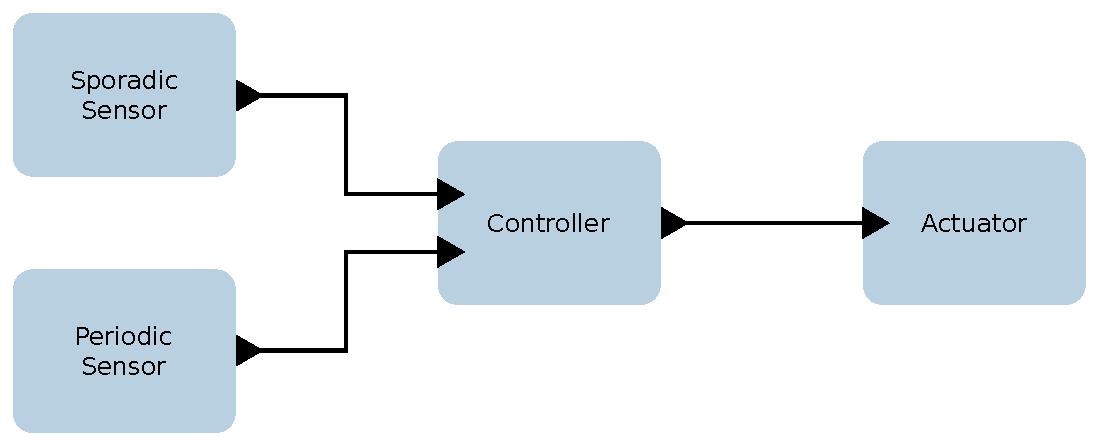
\includegraphics[width=\linewidth]{img/example-2}
 \caption{Second example}
 \label{fig:example-2}
\end{figure}


\subsection{Example 3}
Shut off the lights some time after the switch has been flipped. Reason to have the deadline definition as stated: detectability. Suppose the start deadline cannot be met; the reaction should not be carried out (and the violation be reported on subsequently).

\begin{figure}[ht]
 \centering
 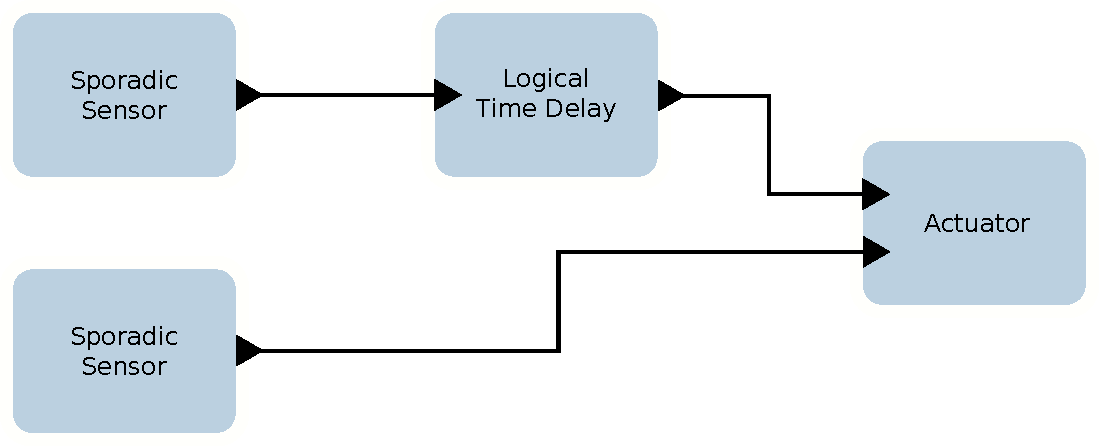
\includegraphics[width=\linewidth]{img/example-3}
 \caption{Third example}
 \label{fig:example-3}
\end{figure}

\marten{In third example, discuss how persistent ports can be used.}
\marten{Also, discuss optimized scheduler that runs ahead of physical time.}
\section{Related Work}
\label{sec:related}

Towards a real-time coordination model for mobile computing \cite{hackmann2005towards}
Method and tools for mixed-criticality real-time applications within PharOS \cite{lemerre2011method}
Accessors \cite{brooks2018component}
S-Net~\cite{grelck2008gentle}
Guarded Atomic Actions~\cite{Rosenband:2004:MSG:996566.996583}
Timed C \cite{Broman_timedC}

Dataflow models are also closely related to the actor approach. In~\cite{wiik2018contract} the authors extend an (untimed) dataflow model with formal contracts that allow guarantees, e.g. for scheduling.
There are timed models of dataflow~\cite{Sriram:00:Scheduling}, and even some structured approaches to use timing semantics in dataflow to execute time-critical applications in cyber-physical systems~\cite{GeilenEtAl:12:Scenarios}.
These models are more restrictive than our propsed work and lack the polyglot flexibility of LF.

Fredlund et al. proposed timed extension of McErlang
as a model checker of timed Erlang programs in \cite{DBLP:conf/forte/EarleF12}. In this extension a new API is introduced to provide the definition and manipulation of time-stamps.
In \cite{DBLP:journals/csur/BoerSHHRDJSKFY17}, de Boar et al. provided a survey on active object languages but there is no focus on timed features.

\martin{Oh boy, we have way too many references for a 4 pages position paper.}
\marjan{That's why I happily didn't add much to the Related Work section. I just wrote the McErlang part, and now I added a line on a survey that can just be commented out for this paper. I think the work of Gul, RTSynchronizer, is very close, although it is very old. Also the Theatre framework is close but can be ignored for now. }
%\section{Actors}
%


% Constraints can be placed on actors' allowable behaviors so that actors adhere to a well-defined model of computation, satisfying desirable properties such as deadlock freedom, schedulability, bounded memory usage, and deterministic execution by construction. This has been the guiding principle in the Ptolemy project\footnote{\url{https://ptolemy.berkeley.edu/}}, which studies modeling, simulation, and design of concurrent, real-time, embedded systems.

% Several frameworks have been built based, loosely or strictly, on the
% original Hewitt actor model
% \cite{Hewitt:77:Actors,Agha:97:ActorComputation}, including Akka
% \cite{AkkaAction2016},
% Ray \cite{DBLP:journals/corr/abs-1712-05889}, and Rebeca
% \cite{DBLP:journals/fuin/SirjaniMSB04}. One property of the original
% Hewitt actor model is that messages received by an actor from distinct
% sources are handled in nondeterministic order. \marten{even messages from the same source can arrive out-of-order}


% \martin{We need to check this: Outputs generated by a time triggered
% reaction are timestamped. When the system is simulated, the timestamp
% is equal to the model time. When the system is used for execution, the logical
% time for the release of the reaction is synchronized to wall clock time and therefore
% the output message are synchronized to wall clock time.}



% \martin{We have (and maybe support) two options: (1) input is only valid when
% the timestamp equals logical time, absent at other times or (2) keeping the value
% of an input for future logical time and having a default value for system initialization time.
% (in the JS accessors this is the way it is specified, the default value gives the
% ``keep'' or persistent semantic).}

\section{The Lingua Franca Compiler Tool Chain}
% Time is \emph{logical} time. This logical time be used for simulation and then
% we call it model time. We can also use the network of actors for the implementation
% of the system. In that case wall clock time is used to timestamp input values
% at sensors. Logical time can never advance further than wall clock time. \marten{Not entirely true: an optimized scheduler can do this under very specific circumstances that we'll elaborate on in the example.}


% The scheduler invokes reactions of actors dependent in inputs with timestamps
% that are equal (or earlier--can this happen?) at logical time $t_1$.
% Logical time cannot advance further than wall clock time $t_w$. If next logical
% time $t_2 > t_w$ the scheduler waits till $t_w \ge t_2$.




\todo{Describe that the single threaded execution of JavaScript enforces
the restriction of the call back not interrupting the reaction.}




For dynamic systems, e.g., an IoT that keeps running, but in different contexts
(e.g., places), we support dynamic reconfiguration of the network of actors.
This may be well supported when targeting a dynamic language such as JavaScript,
but harder to implement in C.

To support reconfiguration we need a more complete language than the configuration
language LF. Therefore, our first iteration of dynamic reconfiguration is done in the
host language JavaScript. In that case, the host language needs access to actors and
ports. However, we can use scopes to having access to those parts of the framework
only in well defined places.

\martin{Will we talk about execution hosts such as PRET machines or Patmos
when targeting C and WCET analysis?}


\section{Conclusions}
\label{sec:conclusion}


\subsection*{Acknowledgments}
The work in this paper was supported in part by the National Science Foundation (NSF),
award \#CNS-1836601 (Reconciling Safety with the Internet) and the iCyPhy Research Center
(Industrial Cyber-Physical Systems, supported by Avast, Camozzi Industries, Denso, Ford, Siemens, and Toyota
%The work presented in this paper was partially funded by the
%Danish Council for Independent Research \textbar{} Technology and Production Sciences
%under the project PREDICT\footnote{\url{http://predict.compute.dtu.dk/}}
%contract no.~4184-00127A.

% Please do not add any references to msbib.bib.
% They get lost when I 'generate' it again.
\bibliographystyle{ACM-Reference-Format}
\bibliography{Refs} 

\end{document}
